\section{The Route It Named Is One of Six}
\label{sec:ch15-the-route-it-named-is-one-of-six}

\index{resolvability!one path printed, several broken|(}%
The composer printed one query. Six more reach the same field without going
anywhere near the Search service, and every one of them is broken in exactly
the same way. Here they are, written as a client would send them, against the
graph as it now stands:

\begin{minted}{graphql}
{ sessions(first: 10) { nodes { averageScore } } }
{ sessions(first: 10) { edges { node { averageScore } } } }
{ sessionById(id: 1) { averageScore } }
{ node(id: "U2Vzc2lvbjox") { ... on Session { averageScore } } }
{ nodes(ids: ["U2Vzc2lvbjox"]) { ... on Session { averageScore } } }
\end{minted}

\index{resolvability!the mutation payload is a route too}%
Five, and the sixth is a mutation. \code{rescheduleSession} returns a payload
carrying a \code{session}, so chapter~\ref{ch:schema-design}'s reschedule is
another way into the type and fails there as well. Add the two Search paths,
under \code{nodes} and under \code{edges}, and this one field is reachable
eight ways. Figure~\ref{fig:ch15-one-route-of-six} draws the six.

\begin{figure}[htbp]
  \centering
  % Six query paths into one contributed field, all of them stopping at the same
% crossing, and the one of the six the composer prints.
%
% Same idiom as figures/tikz/ch01-one-field.tex, which fixes it: 0.4pt strokes,
% the Straight Barb arrowhead, sans-serif scriptsize labels, square corners, no
% fills, black on white. The nearest relative is figures/tikz/ch07-the-walk.tex,
% which draws one of these six as a left-to-right walk and marks the step it
% cannot take with a cross; this figure keeps that cross and stacks six lanes
% against one shared crossing, because what chapter 15 adds to chapter 7 is not
% a new walk but the discovery that there were always several.
%
% Laid out as six lanes rather than six columns for the ordinary reason: the
% paths are of different lengths and read left to right, and six columns of a
% tree at this measure leaves no room for the labels. The seam is one vertical
% rule because here it genuinely is one crossing, which is the difference
% between this picture and the one at figures/tikz/ch14-the-climb-crosses.tex,
% whose comment block records why a single rule was wrong there.
%
% The field on the right is drawn solid and unreached. It exists, it is
% correctly declared, and nothing is wrong with it, which is the point of
% drawing it as an ordinary box rather than as a missing one.
%
% No quotation marks anywhere in this file, including this comment block. SPEC
% decision 30 puts the book in strict Ascii mode and the prose gate reads a
% literal quote character as a quotation mark on sight. Identifiers are bare.
%
% Bare tikzpicture (house style): the figure environment, caption and label
% live at the call site in the section file.
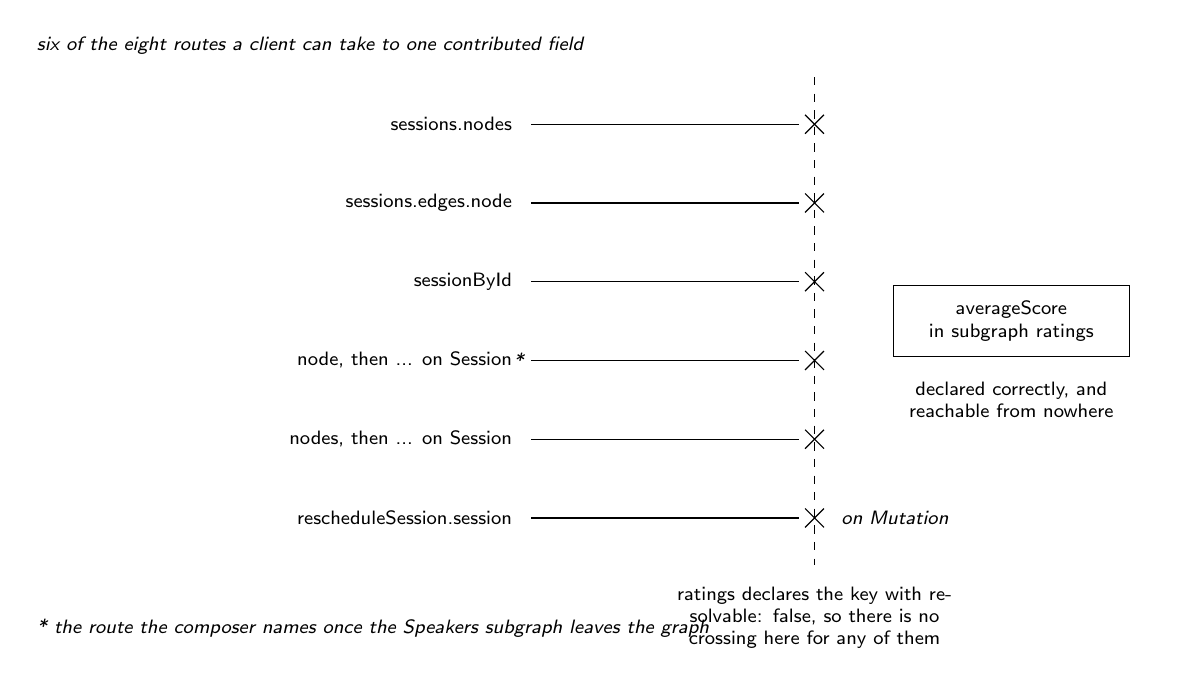
\begin{tikzpicture}[
  x=1mm, y=1mm,
  every node/.append style={font=\sffamily\scriptsize},
  route/.style={draw, line width=0.4pt},
  tick/.style={draw, line width=0.4pt},
  seam/.style={draw, line width=0.4pt, dashed},
  fieldbox/.style={draw, line width=0.4pt, minimum width=30mm,
    minimum height=9mm, align=center, inner sep=1pt},
  path/.style={anchor=east, align=right, inner sep=1pt},
  lane/.style={anchor=west, font=\sffamily\scriptsize\itshape},
  tag/.style={anchor=west, font=\sffamily\scriptsize\itshape, inner sep=1pt},
  spanlabel/.style={anchor=north, align=center, inner sep=2pt},
]

\node[lane] at (0,10)
  {six of the eight routes a client can take to one contributed field};

% ------------------------------------------------------ the six routes
% One lane each, path text on the left, a rule running right to the crossing.
% The cross at the end is chapter 7's buffer stop, and it is at the same x on
% every lane because it is the same crossing every time.
% Paths are written the way the composer writes them, dot-separated, rather
% than with a dash: a double hyphen in a TikZ node is text mode and LaTeX sets
% it as an en dash, which the book does not use anywhere.
\foreach \y/\p in {
    0/{sessions.nodes},
   -10/{sessions.edges.node},
   -20/{sessionById},
   -30/{node, then ... on Session},
   -40/{nodes, then ... on Session},
   -50/{rescheduleSession.session}}{
  \node[path] at (62,\y) {\p};
  \draw[route] (64,\y) -- (98,\y);
  \draw[tick] (98.8,\y-1.2) -- (101.2,\y+1.2);
  \draw[tick] (98.8,\y+1.2) -- (101.2,\y-1.2);
}

% Lane six is on the mutation root rather than on the query root.
\node[tag] at (103,-50) {on Mutation};

% --------------------------------------------------------- the crossing
\draw[seam] (100,6) -- (100,-56);
\node[spanlabel, text width=46mm] at (100,-58)
  {ratings declares the key with resolvable: false, so there is no crossing
   here for any of them};

% ------------------------------------------------------------ the field
\node[fieldbox] (field) at (125,-25) {averageScore\\in subgraph ratings};
\node[spanlabel, text width=34mm] at (125,-32)
  {declared correctly, and reachable from nowhere};

% ------------------------------------------- which one gets reported
% A mark and a legend rather than a change of line style. All six lanes are the
% same walk failing the same way, so nothing about the route itself may be
% drawn differently; what is different is only that this one reached the
% report. Solid against dashed already carries the crossing in this figure and
% the arrowhead already carries a blocked step in ch07-the-walk.tex, so neither
% is available here.
\node[tag, anchor=east] at (63.5,-30) {*};
\node[lane] at (0,-64)
  {* the route the composer names once the Speakers subgraph leaves the graph};

\end{tikzpicture}

  \caption{Six ways to ask for one field, all of them stopping in the same
  place. What each route has to do at its last step is identical: leave the
  subgraph that answered everything before it and enter the one that owns
  \code{averageScore}, through a key that now refuses entry. The composer
  reports one of them and says nothing about the rest, so a fix verified
  against the printed query is a fix verified against an eighth of the problem.
  The two routes through the Search service are not drawn, and in the
  four-service graph one of those is the route the composer prints; the starred
  lane is what it names once Speakers leaves.}
  \label{fig:ch15-one-route-of-six}
\end{figure}

\index{resolvability!the report is per field}%
The composer is not being lazy about five of six. It is answering a different
question from the one the printed query suggests. It asks whether the field can
be reached at all, and prints the route it happened to be standing on when it
gave up. Three errors for three fields, not eighteen for eighteen paths.

\subsection{And the Message Moves When You Are Not Looking}

\index{resolvability!the path depends on the rest of the graph}%
Take Speakers out of \code{graph.yaml} and change nothing else. Same Ratings
document, same defect, same fix, and a service that declares no \code{Session}
at all is the one that left. Here is the path the composer now prints, and the
first of the same four reason lines under it:

\begin{minted}[fontsize=\footnotesize,breakanywhere]{text}
The field "averageScore" is unresolvable at the following path:
 query {
  node {
   ... on Session {
    averageScore <--
   }
  }
 }
This is because:
 - The root type field "Query.node" is defined in the following subgraph: "sessions".
\end{minted}

\index{resolvability!chapter 7's error, one chapter later}%
Which is the error chapter~\ref{ch:composition} printed, arrived at from a
different direction. That chapter composed two documents to produce it. This
one composed three and got the same query out of a graph twice the size, while
the four-service version of the identical defect named something else entirely.
What moved is a service that has nothing to do with either the mistake or the
fix.

\index{graph.yaml@\code{graph.yaml}!its order reaches the message}%
The order of the lines in \code{graph.yaml} reaches the message too. Reverse
the four subgraph entries, leaving the same four documents, and the printed
path does not move but the third of the four reason lines does:

\begin{minted}[fontsize=\footnotesize,breakanywhere]{text}
 - The entity ancestor "Session" in subgraph "search" has no accessible target entities (resolvable @key directives) …
the subgraphs where "Session.averageScore" is defined.
\end{minted}

\index{resolvability!the ancestor named is not on the path}%
\code{search} where it said \code{sessions}, for a query that has not changed.
Both services declare a \code{Session} they cannot enter ratings from, both are
correct to complain, and which of the two ends up in the sentence is decided by
the order I happened to list them in.

\index{wgc@\code{wgc}!the box eats the explanation}%
The ellipsis at the end of that first line is not mine. \code{wgc} draws a
fixed 120-column box around its errors and elides whatever will not fit, so the
longer name has cost the sentence the word \emph{in}. There is no flag that
turns the box off and no structured output to read instead; the four options
the command takes are about warnings, resolvability, external keys and
splitting the config. A tool that formats its own diagnosis to a fixed width
will sometimes eat part of it.

\index{resolvability!two runs of one input agree}%
None of this is nondeterminism. Two runs of the same input are byte for byte
identical, every time. It is stable and it is sensitive to things that are not
about your mistake, which is a worse combination than being flaky, because
flaky gets investigated.
\index{resolvability!one path printed, several broken|)}%
